\documentclass{beamer}
%\usetheme{Ilmenau}
%\usecolortheme{beaver}

\usepackage[slovak,american]{babel}
\usepackage[utf8]{inputenc}
\usepackage{graphicx}
\usepackage{adjustbox}
 \usepackage{xcolor}
 
 \newsavebox\MBox
\newcommand\Cline[2][red]{{\sbox\MBox{$#2$}%
  \rlap{\usebox\MBox}\color{#1}\rule[-2.2\dp\MBox]{\wd\MBox}{1pt}}}

%\usefonttheme{serif}

\definecolor{UKOrange}{HTML}{ef9424} %
\definecolor{UKBrown}{HTML}{a96d5e} %
\definecolor{UKLight}{HTML}{d8b6ab} %
\definecolor{UKDark}{HTML}{7a4f44}
\definecolor{UKDarker}{HTML}{4d312b} 
\definecolor{UKDarkest}{HTML}{2e1e1a}
\definecolor{UKRed}{HTML}{bf1f1c}

\setbeamertemplate{footline}[frame number]{}
\setbeamertemplate{navigation symbols}{}

%\usecolortheme{beaver}
\setbeamertemplate{itemize item}[square]
\setbeamercolor{itemize item}{fg = UKBrown}
\setbeamercolor{itemize subitem}{fg = UKLight}
\setbeamercolor{enumerate item}{fg = UKDark}

\setbeamercolor{footnote}{fg=UKLight}
\setbeamercolor{footnote mark}{fg=UKLight}
\setbeamerfont{footnote}{size=\tiny}
\renewcommand\footnoterule{}

\usetheme{default}
\beamertemplatenavigationsymbolsempty
\setbeamercolor{title}{fg=white, bg=UKBrown}
\setbeamercolor{frametitle}{fg=white, bg=UKBrown}
\setbeamercolor{block title}{bg=UKBrown, fg= white}
\setbeamercolor{block body}{bg =UKLight, fg = UKDarkest}

\useoutertheme[subsection=false]{miniframes}
\AtBeginSection[]{\subsection{}}

\setbeamercolor{below lower separation line head}{bg=UKDark}
\addtobeamertemplate{headline}{}{%
  \begin{beamercolorbox}[colsep=0.5pt]{below lower separation line head}
  \end{beamercolorbox}
}
%\setbeamercolor*{mini frame}{fg=white,bg=UKRosy}
\setbeamercolor{section in head/foot}{fg=UKLight, bg=UKDark}

%\setbeamertemplate{itemize/enumerate body begin}{\normalsize}
%\setbeamertemplate{itemize/enumerate subbody begin}{\normalsize}




%\newcommand{\codeblock}[2]{ \begin{block}{#1} \begin{verbatim}#2\end{verbatim}\end{block}}

%\defbeamertemplate*{title page}{customized}[1][]
%{
%  \begin{centering}
%    \begin{beamercolorbox}[sep=8pt,center]{title}
%      \usebeamerfont{title}\inserttitle
%    \end{beamercolorbox}
%  \end{centering}
%  \bigskip
%
%\begin{columns}[onlytextwidth,T]
%
%
%  \column{27mm}
%  \includegraphics[width=27mm]{images/logoFMFI.png}
%  
%  \column{\dimexpr\linewidth-54mm-6mm}
%  \centering
%  \vspace{5mm}  
%  \usebeamerfont{author}\insertauthor\par
%  \vspace{5mm}
%  \usebeamerfont{institute}\insertinstitute\par
%
%  \column{27mm}
%  \includegraphics[width=27mm]{images/logoUK.png}  
%\end{columns}
%\centering
%\vspace{7mm}
%  \usebeamerfont{date}\insertdate\par
%}


\title[Príznaky]{Rozpoznávanie obrazcov - 3. cvicečenie \\ Štatistika II.}
\author[Viktor Kocur]{Viktor Kocur \\{\small viktor.kocur@fmph.uniba.sk}}
\institute{DAI FMFI UK}
\date{2.3.2020}
%\titlegraphic{\includegraphics[width=2.7cm]{images/logoFMFI.png}\hspace*{1cm}~%
%   \includegraphics[width=2.7cm]{images/logoUK.png}
%}


\begin{document}
\selectlanguage{slovak}

\begin{frame}[plain]
  \titlepage  
\end{frame}

\section{Distribučná funkcia}
%\subsection{Introduction}

\begin{frame}
\frametitle{Náhodná premenná}

\begin{block}{Náhodná premenná}
Funkcia, ktorej hodnota je určená výsledkom náhodného pokusu. Priraďuje číselnú hodnotu každému javu.
\end{block}

\begin{block}{Distribučná funkcia}
Distribučná funkcia - opisuje rozdelenie pravdepodobnosti náhodnej premennej definovanej na pravdepodobnostnom priestore.
\end{block}
\end{frame}

\begin{frame}
\frametitle{Distribučná funkcia}

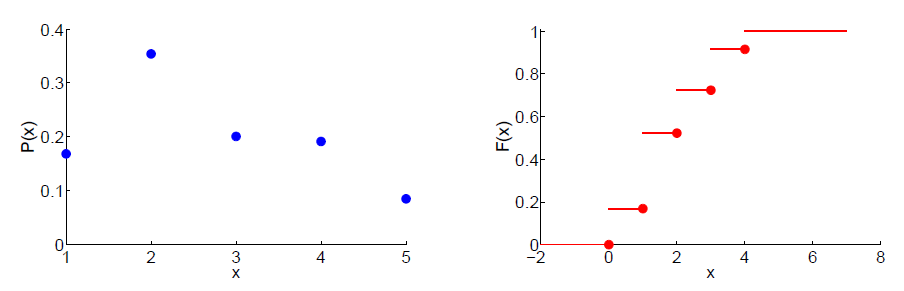
\includegraphics[width=\textwidth]{df1.png}

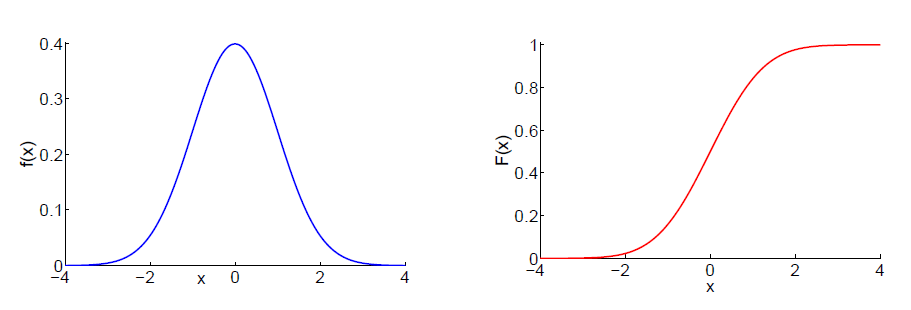
\includegraphics[width=\textwidth]{df2.png}
\end{frame}


\section{Bernoulliho schéma}
\begin{frame}
\frametitle{Bernoulliho schéma}

\begin{block}{Bernoulliho schéma}
Uvažujeme $n$ na sebe nezávislých pokusov. Pradvdepodobnosť úspechu v každom z nich je $p$. Potom pre premennú $X$ ktora označuje počet úspečných pokusov platí:

\begin{equation}
P(X = k) = \binom{n}{k} p^k (1 - p)^{n-k} 
\end{equation}
\end{block}
\end{frame}

\begin{frame}
\frametitle{12. Príklad}

Študent má vypracovať test, ktorý obsahuje 10 otázok a ku každej z nich sú 4 odpovede, pričom práve jedna je správna. Aké sú pravdepodobnosti, že študent, ktorý látku vôbec nepozná a volí odpovede náhodne, zodpovie správne a) aspoň 5 otázok b) najviac 5 otázok

Riešenie a)
\begin{itemize}
\item<2-> $P(A) = P(X = 5) + P(X = 6) + P(X = 7) + P(X = 8) + P(X = 9) + P(X = 10)$
\item<3-> $P(X = 5) = \binom{10}{5} 0.25^5 \cdot 0.75^5$
\item<4-> $P(A) = \sum_{k=5}^{10} \binom{10}{k} 0.25^k \cdot 0.75^{10-k}$
\end{itemize}

\end{frame}

\begin{frame}
\frametitle{13. Príklad}

Asi 75\% zahraničným turistom chutia naše bryndzové halušky. Aká je pravdepodobnosť, že z 20 zahraničných hostí si a) aspoň 17 na haluškách pochutí, b) že halušky budú chutiť všetkým hosťom?

\begin{itemize}
\item<2-> $P(A) = P(X = 17) + P(X = 18) + P(X = 19) + P(X = 20)$
\item<3-> $P(X = 20) = \binom{20}{20} 0.75^{20} \cdot 0.25^0 = 0.75^{20}$
\item<4-> $P(A) = \sum_{k=17}^{20} \binom{10}{k} 0.75^k \cdot 0.25^{10-k}$
\end{itemize}
\end{frame}

\section{Parametre rozdelenia}


\begin{frame}
\frametitle{Štandardná odchylka}
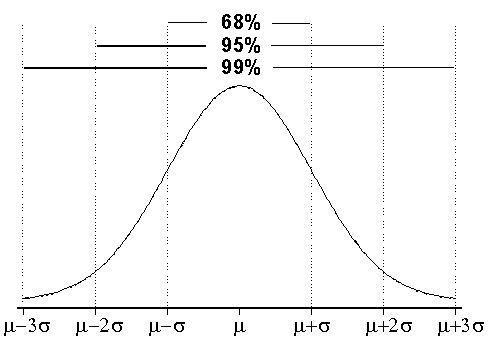
\includegraphics[width = \textwidth]{df3.png}
\end{frame}

\begin{frame}
\frametitle{Odhad parametrov rozdelení}

\begin{block}{Výberový priemer}
$ \overline{X} = \frac{1}{n} \sum_{i=1}^n X_i $
\end{block}

\begin{block}{Výberový rozptyl}
$ S^2 = \frac{1}{n-1} \sum_{i=1}^n (X_i - \overline{X})^2 $
\end{block}


\begin{block}{Smerodajná odchýlka}
$S = \sqrt{S^2}$
\end{block}

\begin{block}{Výberová kovariancia}
$S_{XY} = \frac{1}{n-1} \sum_{i=1}^n (X_i - \overline{X})(Y_i - \overline{Y}) $
\end{block}
\end{frame}

\begin{frame}
\frametitle{Odhad parametrov rozdelení}

\begin{block}{Intervalový odhad spoľahlivosti}
$P (G_D < \theta < G_H) = 1 - \alpha$
\end{block}

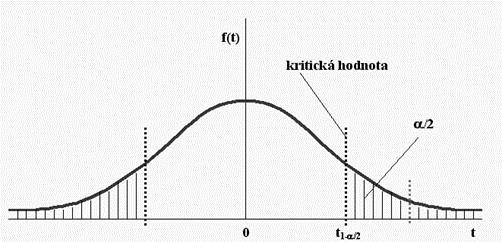
\includegraphics[width=\textwidth]{df4.png}
\end{frame}


\begin{frame}
\frametitle{Odhad parametrov rozdelení}

\begin{table}[t]
\begin{tabular}{|l|c|c|c|c|c|}
\hline
$\alpha$     & 0.01   & 0.02   & 0.05   & 0.1    & 0.2   \\ \hline
$u_{\alpha/2}$ & 2.5758 & 2.3263 & 1.9599 & 1.6448 & 1.299 \\ \hline
\end{tabular}
\end{table}
\begin{equation*}
X \sim N(0,1) P(|X| > u_{\alpha/2}) = \alpha
\end{equation*}

\begin{align*}
1 - \alpha &= P(-u_{\alpha/2} < U < u_{\alpha/2}) \\
               &= P(-u_{\alpha/2} < \frac{\overline{X}-\mu}{\sigma} < u_{\alpha/2}) \\
               &= P(\overline{X} - u_{\alpha/2} \cdot \frac{\sigma}{\sqrt{n}} < \mu < \overline{X} + u_{\alpha/2} \cdot \frac{\sigma}{\sqrt{n}})
\end{align*}

\end{frame}


\begin{frame}
\frametitle{Testovacie štatistiky}

Ak poznáme hodnotu $\sigma$ originálnej distribúcie. Potom používame normálnu distribúciu:

\begin{equation*}
u = \frac{\overline{X} - \mu_0}{\frac{\sigma}{\sqrt{n}}}
\end{equation*}

Ak ju nepoznáme, tak pre $n > 30$ použijeme:

\begin{equation*}
u = \frac{\overline{X} - \mu_0}{\frac{S}{\sqrt{n}}}
\end{equation*}

Ak je $n < 30$, tak použieje Študentovu distribúciu pre:

\begin{equation*}
t = \frac{\overline{X} - \mu_0}{\frac{S}{\sqrt{n}}}
\end{equation*}

\end{frame}


\begin{frame}
\frametitle{Testovacie štatistiky - Matlab}

\begin{block}{Hodnoty $u_{\alpha}$ a $t_{\alpha}$}
Kritické hodnotenia je možé zistiť z tabuliek. My to budeme robiť pomocou matlabu.
\end{block}

\begin{block}{norminv}
norminv(alpha) - vráti kritickú hodnotu pre hladinu alpha pre normálne rozdelenie
\end{block}

\begin{block}{tinv}
tinv(alpha, n) - vráti kritickú hodnotu pre hladinu alpha pre Študentovo rozdelenie pre výberový súbor s n stupňami volnosti.
\end{block}

\begin{block}{Poznámka}
Ak chceme napr. obojstranný interval spoľahlivosti 0.95, tak ako alpha použijeme 0.975, resp. [0.025, 0.0975].
\end{block}
\end{frame}

\begin{frame}
\frametitle{14. Príklad}

Predpokladáme, že výška chlapcov vo veku 9-10 rokov má normálne rozdelenie s neznámou strednou hodnotou a odchýlko $\sigma^2 = 39.112$. Zmerali sme výšku 15 chlapcov a určili výberovú strednú hodnotu 139.13 cm. Určite 99\% obojstranný interval spolahlivosti.

\begin{itemize}
\item<2-> $n = 15, \sigma  = 6.253, \overline{X} = 139.13$
\item<3-> $1 - \alpha = P(\overline{X} - u_{\alpha/2} \cdot \frac{\sigma}{\sqrt{n}} \leq \mu \leq \overline{X} + u_{\alpha/2} \cdot \frac{\sigma}{\sqrt{n}})$
\item<4-> $139.13 \pm 2.5758 \cdot \frac{6.253}{\sqrt{15}}$
\item<5-> $134.97 \leq \mu \leq 143.28$
\end{itemize}
\end{frame}


\begin{frame}
\frametitle{15. Príklad}
Letecká spoločnosť odhaduje priemerný počet cestujúcich. V priebehu 20 dní bol priemerný počet cestujúcich 112 s výberovým rozptylom 25. Nájdite 95\%-ný obojstranný interval spoľahlivosti pre priemerný počet cestujúcich $\mu$.

\begin{itemize}
\item<2-> $n = 20, S  = 5, \overline{X} = 112$
\item<3-> $1 - \alpha = P(\overline{X} - t_{\alpha/2, n-1} \cdot \frac{S}{\sqrt{n}} \leq \mu \leq \overline{X} + t_{\alpha/2, n-1} \cdot \frac{S}{\sqrt{n}})$
\item<4-> $112 \pm 2.093 \cdot \frac{5}{\sqrt{20}}$
\item<5-> $109.65 \leq \mu \leq 114.34$
\end{itemize}
\end{frame}


\begin{frame}
\frametitle{16. Príklad}
Náhodná premenná X má normálne rozdelenie, kde stredná hodnota aj odchýlka sú neznáme. Namerané realizácie $X$ sú 27, 15, -3, -6, 12, 20, 13, 0, 7, 10. Zistite 95\%-ný obojstranný interval spoľahlivosti pre strednú hodnotu.

\begin{itemize}
\item<2-> $n = 10, S  = 10.319, \overline{X} = 9.5$
\item<3-> $1 - \alpha = P(\overline{X} - t_{\alpha/2, n-1} \cdot \frac{S}{\sqrt{n}} \leq \mu \leq \overline{X} + t_{\alpha/2, n-1} \cdot \frac{S}{\sqrt{n}})$
\item<4-> $9.5 \pm 2.262 \cdot \frac{10.319}{\sqrt{10}}$
\item<5-> $2.118 \leq \mu \leq 16.881$
\end{itemize}
\end{frame}

\begin{frame}
\frametitle{17. Príklad}

Zo základného súboru s normálnym rozdelením, kde je známy rozptyl $\sigma^2 = 0.06$ sme urobili náhodný výber s prvkami 1.3, 1.8, 1.4, 1.2, 0.9, 1.5, 1.7. Zistite 95\% interval spoľahlivosti pre strednú hodnotu $\mu$.

\begin{itemize}
\item<2-> $n = 7, \sigma  = 0.245, \overline{X} = 1.4$
\item<3-> $1 - \alpha = P(\overline{X} - u_{\alpha/2} \cdot \frac{\sigma}{\sqrt{n}} \leq \mu \leq \overline{X} + u_{\alpha/2} \cdot \frac{\sigma}{\sqrt{n}})$
\item<4-> $1.4 \pm 1.9599 \cdot \frac{0.245}{\sqrt{7}}$
\item<5-> $1.218 \leq \mu \leq 1.581$
\end{itemize}
\end{frame}

\begin{frame}
\frametitle{Testovanie hypotéz - Matlab}

\begin{block}{ztest}
[h, p, ci] = ztest(X, m, sigma, 'Alpha', alpha) - vráti výsledok testu pre hypotézu, že dáta vo vektore $X$ sú z normálnej distribúcie so strednou hodnotou $m$ a štandardnou odchýlkou $sigma$. $h$ obsahuje 1 ak sa hypotéza nepotrvdí pre danú úroveň významnosti $alpha$, inak 0, $ci$ obsahuje interval spoľahlivosti.
\end{block}

\begin{block}{ttest}
[h, p, ci] = ttest(X, m, 'Alpha', alpha) - vráti výsledok testu pre hypotézu, že dáta vo vektore $X$ sú z normálnej distribúcie so trednou hodnotou $m$ a a neznámou štandardnou odchýlkou. $h$ obsahuje 1 ak sa hypotéza nepotrvdí pre danú úroveň významnosti $alpha$, inak 0, $ci$ obsahuje interval spoľahlivosti.
\end{block}

\begin{block}{Úloha}
Otestujte ztest funkciu na 16. a 17. príklad.
\end{block}
\end{frame}

\begin{frame}
\frametitle{18. Príklad}

Tvrdíme, že guľôčky vyrobené automatickým sústruhom, majú strednú hodnotu polomeru 10mm. Použitím obojstranného testu významnosti na hladine 0.05 otestujte túto hypotézu ak vo výbere zo 16 guľôčok je priemer ich polomerov 10.3 mm a a) $\sigma^2 = 1$, b) $S^2 = 1.21$. 

Riešenie a)
\begin{itemize}
\item<2-> $n =16, \sigma = 1, \overline{X} = 10.3$
\item<3-> $1 - \alpha = P(\overline{X} - u_{\alpha/2} \cdot \frac{\sigma}{\sqrt{n}} \leq \mu \leq \overline{X} + u_{\alpha/2} \cdot \frac{\sigma}{\sqrt{n}})$
\item<4-> $10.3 \pm 1.9599 \cdot \frac{1}{\sqrt{16}}$
\item<5-> $9.81 \leq \mu \leq 10.789$
\item<5-> Hypotézu nezamietneme
\end{itemize}
\end{frame}

\begin{frame}
\frametitle{18. Príklad}

Tvrdíme, že guľôčky vyrobené automatickým sústruhom, majú strednú hodnotu polomeru 10mm. Použitím obojstranného testu významnosti na hladine 0.05 otestujte túto hypotézu ak vo výbere zo 16 guľôčok je priemer ich polomerov 10.3 mm a a) $\sigma^2 = 1$, b) $S^2 = 1.21$. 

Riešenie b)
\begin{itemize}
\item<2-> $n =16, S = 1.1, \overline{X} = 10.3$
\item<3-> $1 - \alpha = P(\overline{X} - t_{\alpha/2, n-1} \cdot \frac{S}{\sqrt{n}} \leq \mu \leq \overline{X} + t_{\alpha/2, n-1} \cdot \frac{S}{\sqrt{n}})$
\item<4-> $10.3 \pm 2.131 \cdot \frac{1.1}{\sqrt{16}}$
\item<5-> $9.71 \leq \mu \leq 10.88$
\item<5-> Hypotézu nezamietneme
\end{itemize}
\end{frame}







\end{document}